\documentclass[conference]{IEEEtran}
\usepackage{times}

% numbers option provides compact numerical references in the text.
\usepackage[numbers]{natbib}
\usepackage{multicol}
\usepackage[bookmarks=true]{hyperref}
\usepackage{amsmath,amssymb}
% \usepackage[standard]{ntheorem}
\usepackage{amsthm}
\usepackage{mathtools}
\usepackage{bm}
\usepackage{graphicx}
% \usepackage{caption}
% \usepackage{figure}
\usepackage{float}
\usepackage{subcaption}
\usepackage{epstopdf}
\usepackage{dblfloatfix}
\usepackage{fixltx2e}
% \usepackage{subfig}
\usepackage{mathrsfs}
\usepackage{algorithm}
\usepackage{algorithmicx}
\usepackage[noend]{algpseudocode}
\makeatletter
\def\BState{\State\hskip-\ALG@thistlm}
\makeatother
\algdef{SE}[DOWHILE]{Do}{DoWhile}[1]{\algorithmicdo\ #1}[1]{\algorithmicwhile\ #1}

\usepackage{booktabs}
\newcommand\Tstrut{\rule{0pt}{2.5ex}}       % "top" strut
\newcommand\Bstrut{\rule[-0.9ex]{0pt}{0pt}} % "bottom" strut
\newcommand{\TBstrut}{\Tstrut\Bstrut} % top&bottom struts

\usepackage{tabstackengine}
\stackMath

\usepackage{tikz}
\usetikzlibrary{scopes}
\usetikzlibrary{shapes.misc}
\tikzset{cross/.style={cross out, draw=black, minimum size=2*(#1-\pgflinewidth), inner sep=0pt, outer sep=0pt},
%default radius will be 1pt.
cross/.default={2pt}}

\let\labelindent\relax
\usepackage{enumitem}
% \newenvironment{enum}{\begin{enumerate}[wide, labelwidth=!, labelindent=0pt]}{\end{enumerate}}
\newlist{inparaenum}{enumerate}{2}% allow two levels of nesting in an enumerate-like environment
\setlist[inparaenum]{nosep,wide,labelwidth=!,labelindent=0pt}% compact spacing for all nesting levels
\setlist[inparaenum,1]{label=\bfseries\arabic*)}% labels for top level
\setlist[inparaenum,2]{label=\arabic{inparaenumi}{\alph*})}% labels for second level

\newtheorem{theorem}{Theorem}
\newtheorem{proposition}{Proposition}
\newtheorem{definition}{Definition}
\newtheorem{corollary}{Corollary}
\newcommand\numberthis{\addtocounter{equation}{1}\tag{\theequation}}
\DeclareMathOperator{\sign}{\text{sgn}}
\DeclareMathOperator*{\argmin}{arg\,min}
\DeclareMathOperator{\intr}{int}
\DeclareMathOperator{\dom}{dom}
\DeclareMathOperator{\rot}{\text{rot}}

\newcommand{\BB}[1]{{\color{red} {Byron: {#1}}}}

\newcommand{\EH}[1]{{\color{blue} {Eric: {#1}}  }}
\newcommand{\AB}[1]{{\color{cyan} {Ankit: {#1}}  }}
\newcommand{\TODO}[1]{{\color{red} {{#1}}  }}

\pdfinfo{
   /Author (Eric Huang)
   /Title  (Robots: Our new overlords)
   /CreationDate (D:20161016120000)
   /Subject (Robots)
   /Keywords (Robots;Overlords)
}

\begin{document}

% paper title
\title{\huge Exact Bounds on the Contact Driven Motion of a Sliding
  Object, With Applications to Robotic Pulling}

% You will get a Paper-ID when submitting a pdf file to the conference system
% \author{Author Names Omitted for Anonymous Review. Paper-ID [65]}

% \author{\authorblockN{}
% \authorblockA{School of Electrical and\\Computer Engineering\\
% Georgia Institute of Technology\\
% Atlanta, Georgia 30332--0250\\
% Email: mshell@ece.gatech.edu}
% \and
% \authorblockN{Homer Simpson}
% \authorblockA{Twentieth Century Fox\\
% Springfield, USA\\
% Email: homer@thesimpsons.com}
% \and
% \authorblockN{James Kirk\\ and Montgomery Scott}
% \authorblockA{Starfleet Academy\\
% San Francisco, California 96678-2391\\
% Telephone: (800) 555--1212\\
% Fax: (888) 555--1212}}

% avoiding spaces at the end of the author lines is not a problem with
% conference papers because we don't use \thanks or \IEEEmembership

% for over three affiliations, or if they all won't fit within the width
% of the page, use this alternative format:
% 
\author{\authorblockN{Eric Huang\authorrefmark{1},
Ankit Bhatia\authorrefmark{1},
Byron Boots\authorrefmark{2} and
Matt Mason\authorrefmark{1}}
\authorblockA{\authorrefmark{1}Robotics Institute\\
Carnegie Mellon University,
Pittsburgh, Pennsylvania 15213\\ Email: \{erich1,ankitb\}@andrew.cmu.edu, matt.mason@cs.cmu.edu}
\authorblockA{\authorrefmark{2}Interactive Computing\\
Georgia Institute of Technology,
Atlanta, Georgia 30332\\ Email: bboots@cc.gatech.edu}}

\maketitle

\begin{abstract}
  This paper explores the quasi-static motion of a planar slider being
  pushed or pulled through a single contact point assumed not to
  slip. The main contribution is to derive a method for computing
  exact bounds on the object's motion for classes of pressure
  distributions where the center of pressure is known but the
  distribution of support forces is unknown. The second contribution
  is to show that the exact motion bounds can be used to plan robotic
  pulling trajectories that guarantee convergence to the final
  pose. The planner was tested on the task of pulling an acrylic
  rectangle to random locations within the robot workspace. The
  generated plans were accurate to 4.00mm $\pm$ 3.02mm of the target
  position and 4.35 degrees $\pm$ 3.14 degrees of the target
  orientation.

  % \EH{TODO: Experimental results} 

  % The distance between the upper and lower motion bounds were 
  % 5-10$\times$ 

  % The exact bounds were shown to 

  % The exact motion bounds an tighter over wide range of object
  % geometries.

% Major contributions:
%   \begin{enumerate}
%   \item Proof of stability
%   \item first known algorithm that computes exact angular velocity
%     bounds on the friction dominated motion of a pushed/pulled object.
%   \item Uncertainty bounds on the orientation
%   \item Planner that exploits the stability of pulling using the exact
%     angular velocity bounds.
%   \item to return trajectories.
%   \item An easy to implement in both hardware and software skill. 
%   \item validated on a real robotic system.
%     A useful addition to a roboticist's toolkit. that is serviceable
%     in a wide range of scenarios. ranging from furniture rearrangement
%     or table-top manipulation to bin picking.
%   \end{enumerate}
\end{abstract}

\IEEEpeerreviewmaketitle

\section{Introduction}

% \TODO{
% Items that an introduction should address:
% \begin{enumerate}
% \item What is the problem?
% \item Why should people care?
% \item What are the major contributions?
% \item What is the structure of this paper?
% \end{enumerate}
% }

% In this paper, we demonstrate the value of 

% \begin{enumerate}
% \item Looking at pushing from a different perspective
% \item contributions
% \item open-loop stable with convergence guarantees
% \item easy to use
% \item Outline of sections
% \end{enumerate}

% \begin{inparaenum}
% \item 

Pushing (or pulling) planar objects with fixed contact is difficult to
model in both theory and practice. First, pressure distributions of
objects are statically indeterminant (barring the case of three-point
support with known center of mass). Second, surface imperfections lead
to spatial variability in both the pressure distribution and
coefficient of friction \cite{YuBFR16}. Though several force-motion
models for pushing exist
\cite{zhou2016convex,howe1996practical,goyal1991planar}, the above
sources of indeterminacy ultimately lead to errors in the predicted
velocity of the pushed object.

If the motion cannot be predicted, then another option is to find
bounds on the velocity of the pushed object. This problem was first
raised in Mason's thesis on robotic pushing \cite{Mason1982}. In the
case of fixed contact pushing, this is equivalent to finding bounds on
angular velocity of the object as it is pushed through the contact
point. To this end, we develop the first algorithm that finds
\textit{exact} angular velocity bounds on the object's motion over all
pressure distributions with shared center of pressure. Moreover, the
bounds are exact for many additional classes of pressure distributions
that have not been considered before.

Dealing with uncertainty is a fundamental challenge in robotics
\cite{Thrun2005}. We demonstrate how our bounds can be applied to
planning for robotic pulling under action uncertainty. Robotic pulling
is a general-purpose manipulation skill for positioning and orienting
objects. The proposed planner uses the angular velocity bounds to find
actions that reduce the uncertainty in the system, i.e. close the
distance between the integrated orientation bounds. Moreover, given a
suitable initialization, the planner finds trajectories that guarantee
the uncertainty at the final pose converges to a very small value.

The rest of the paper is organized as follows. Section
\ref{sec:theory} develops several theoretical results needed to prove
the correctness of our algorithmic contributions. Section
\ref{sec:methods} introduces the exact angular velocity bound
algorithm and the algorithm for planning pulling trajectories under
action uncertainty. Section \ref{sec:experiments} presents our
experimental results. Section \ref{sec:conclusion} gives concluding
remarks on the paper.

\section{Theory}\label{sec:theory}

This section covers our theoretical contributions. Subsection
\ref{sec:prop-angular-velocity-bounds} lays the theoretical groundwork
necessary for proving the correctness of the exact angular velocity
bound algorithm introduced in
\ref{sec:exact-ang-vel-bound-alg}. Subsection
\ref{sec:orientation-bounds} extends the angular velocity bounds to
orientation bounds. This last subsection is mainly to establish
convergence guarantees for robotic pulling trajectories.

% Lastly, \ref{sec:stability} contains a proof of
% the existence and uniqueness (modulo $2\pi$) of a stable equilibrium
% when pulling an object. 

\subsection{Properties of Angular Velocities Bounds}\label{sec:prop-angular-velocity-bounds}

% \EH{Comment: First proposition probably very unnecessary. Removable or
%   shortened.}
% \begin{proposition}
%   The constrained frictional dissipation equation
%   $\mathrm{D}_{\mathcal{C}}(\mathbf{v}^+)$ has a unique minimizer for
%   pressure distributions with some support force off of the
%   $x$-axis. When otherwise, the equation admits an interval of
%   minimizers.
% \end{proposition}

% \begin{proof}
%   The work of \cite{Mason1982} was the first to prove the above
%   observation for finite pressure distributions. For the case of
%   infinite (discrete) pressure distributions, we can appeal to the
%   convexity properties of $\lVert A(\mathbf{x})\mathbf{v}^+ \rVert$.

%   Minkowski's inequality gives
%   $\lVert x + y \rVert \leq \lVert x \rVert + \lVert y \rVert$ with
%   equality if and only if $x$ and $y$ are positively linearly
%   dependent. For two generalized velocities
%   $\mathbf{v}^+_1,\mathbf{v}^+_2\in \mathcal{C}$, the resulting body
%   point velocities are linearly dependent if and only if the
%   determinant
%   \begin{align}
%     \det A(\mathbf{x})
%       \begin{bmatrix*}
%         \mathbf{v}^+_1 & \mathbf{v}^+_2
%       \end{bmatrix*}
%     &= \det
%      \begin{bmatrix*}
%        -x_2\omega_1 & -x_2\omega_2 \\
%        1 + x_1\omega_1 & 1 + x_1\omega_2 
%      \end{bmatrix*}\\
%     &= -x_2(\omega_1 - \omega_2)
%   \end{align}
%   is zero. We immediately see that
%   $\lVert A(\mathbf{x})\mathbf{v}^+ \rVert$ is strictly convex
%   relative to $\mathcal{C}$ if and only if the body point $\mathbf{x}$
%   lies off of the $x$-axis. The proposition follows from the fact that
%   the positive sum of convex functions and a strictly convex function
%   is strictly convex.
% \end{proof}

% An object whose contact region is two discrete points, e.g. a spoon,
% can have multiple minimizing angular velocities when aligned with the
% $x$-axis.

We prove that the set of feasible angular velocities for an object
with known center of pressure is connected and bounded. These two
properties justify the use of a bisection search to locate the minimum
and maximum angular velocities in Subsection
\ref{sec:exact-ang-vel-bound-alg}.

% We begin by citing a proposition from variational analysis used in our
% proofs of the main results.
% \begin{proposition}\label{prop:var-analysis}
%   Suppose $P(u) := \argmin_x f(x,u)$ with
%   $f:\mathcal{X}\times\mathcal{U}\rightarrow\mathbb{R}$ continuous and
%   level-bounded in $x$ locally uniformly in $u$. Then the set-valued
%   mapping $P(u)$ is outer-semicontinuous and locally bounded.
% \end{proposition}

% \begin{proof}
%   Proposition adapted from Corollary 7.42 and Theorem 1.17 in
%   \cite{Rockafellar}.
% \end{proof}

\begin{theorem}\label{thm:angular-velocities}
  For pulling of a planar rigid body with known center of pressure,
  the set of all feasible angular velocities is connected.
\end{theorem}

\begin{proof}
  See \cite{Huang2015Bounds}.
\end{proof}

In general, Theorem \ref{thm:angular-velocities} holds for any convex
set of pressure distributions with known center of pressure. 

% Note, the set of pressure
% distributions with identical centers of pressure is convex.

\begin{corollary}\label{cor:bounded}
  For pulling of a planar rigid body with known center of pressure,
  the set of all feasible angular velocities is a bounded interval.
\end{corollary}

\begin{proof}
  See \cite{Huang2015Bounds}.
\end{proof}

\subsection{Integrated Orientation Bounds}\label{sec:orientation-bounds}

\begin{figure}[t]
  \centering
    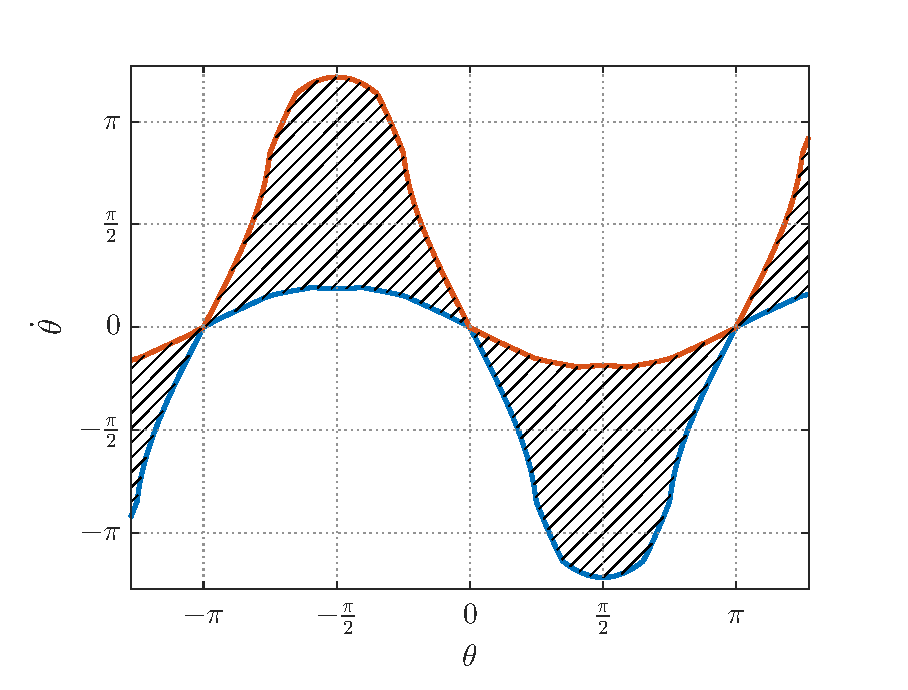
\includegraphics[width=1\linewidth]{fig/omega_bounds_1}
    \caption{Example angular velocity bounds for a 2D object. The
      object is oriented such that the stable pulling configuration
      corresponds to $\theta=0$. The orange curve is the upper bound
      $\alpha$. The blue curve is the lower bound $\beta$.}
  \label{fig:omega-bounds}
\end{figure}

The angular velocity bounds derived in Subsection
\ref{sec:prop-angular-velocity-bounds} can be integrated into bounds
on the position of the pulled body.  Let $\theta$ be the true
orientation of the pulled body in the world frame.  We define the
\textit{angular deviation} of the object as the angle deviation from
the stable pulling configuration in the frame of the moving contact
point. A deviation of 0 degrees corresponds to the center of pressure
dragging behind the contact point.
% In Figure \ref{fig:presspull-motion}, the rectangular object has an
% angular deviation of 135 degrees.
Let the function $\omega$ map from the
angular deviation to the true angular velocity. Likewise, let $u$ and
$l$ be upper and lower bounds on the true orientation, and let the
functions $\alpha$ and $\beta$ map from the angular deviation to the
upper and lower angular velocity bound. An example plot of $u$ and $l$
is illustrated in Figure \ref{fig:omega-bounds}.

We assume that the pulling trajectory
$\gamma:\mathbb{R}\rightarrow\mathbb{R}^2$ can be approximated by a
finite number of straight line segments of equal length. Given such a
$\gamma$, the pulling angle
$\phi(t) = \tan^{-1}(\dot{\gamma}_y(t),\dot{\gamma}_x(t))$ is a
piece-wise constant (step) function. Let
$v(t) = \lVert\dot{\gamma}(t)\rVert$. As the planar rigid body is
pulled along $\gamma$ with unit velocity, the state and bounds change
according to the dynamical system
\begin{align}
  \dot{x} &= \cos(\phi(t))\\
  \dot{y} &= \sin(\phi(t))\\
  \dot{\theta} &= \omega(\theta - \phi(t) + \pi)\\
  \dot{u} &=  \alpha(u - \phi(t) + \pi) \label{eq:u-ode}\\ 
  \dot{\ell} &=  \beta(\ell - \phi(t) + \pi). 
\end{align}

\begin{proposition}\label{prop:orientation-bounds}
  For pulling of a rigid body with known initial pose, the orientation
  of the body is bounded above and below by $u$ and $\ell$.
\end{proposition}

\begin{proof}
  See \cite{Huang2015Bounds}.
\end{proof}

\section{Methods}\label{sec:methods}

In this section, we synthesize the materials in Section
\ref{sec:theory} into an algorithm for computing exact angular
velocity bounds and a method for planning convergent trajectories
using the computed bounds. The former is detailed in Subsection
\ref{sec:exact-ang-vel-bound-alg} and extended in Subsection
\ref{sec:point-in-moment-enve} and the latter is detailed in
Subsection \ref{sec:diff-dynam-progr}.

% The first subsection, \ref{sec:point-in-moment-enve}, details the
% changes to the moment hull (Subsection \ref{sec:frictional-envelope})
% that facilitate computations over a new class of pressure-distribution
% assumptions.

% Subsection \ref{sec:diff-dynam-progr} applies the exact angular
% velocity bounds to planning pulling trajectories using Differential
% Dynamic Programming (DDP).

\subsection{Exact Angular Velocity Bound
  Algorithm}\label{sec:exact-ang-vel-bound-alg}

\begin{algorithm}[t]
\caption{Exact Angular Velocity Bounds}\label{alg:angular-velocity-bounds}
\begin{algorithmic}[1]
\Function{Find Extrema}{$R$, $x_0$, $y_0$}
\If {$x_0$ is $0$} \Return {$[0,0]$}
\EndIf
% \BState \emph{min}:
\State $P \gets \min_\mathbf{x} \mathbf{0} \text{\;s.t.\;} R\mathbf{x} = [x_0,y_0]^T,  L \leq \mathbf{x} \leq U$
\State $x_r \gets \Call{Compute Rotation Center}{R,P}$
\State $l \gets 0$
\State $u \gets -\lVert\mathbf{v}_c\rVert/x_r$
\State $\omega_1 \gets \Call{Bisection Search}{R,x_0,y_0,l,u}$
% \BState \emph{max}:
\State $l \gets u \gets -\lVert\mathbf{v}_c\rVert/x_r$
\Do% {$u \gets 2u$}
\State {$l \gets 2l$}
\State $\mathbf{v}^+ \gets [\mathbf{v}_c^T, l]^T$
\State $G \gets \{-\mathbf{x}\times A(\mathbf{x})\mathbf{v}^+ / \lVert A(\mathbf{x})\mathbf{v}^+ \rVert \;|\; \mathbf{x} \in R\}$
\DoWhile{$[x_0,y_0,0]^T \in \Call{ConvHull}{G}$}
\State $\omega_2 \gets \Call{Bisection Search}{R,x_0,y_0,l,u}$
% \BState \emph{return}:
\State $l \gets \Call{Min}{\omega_1,\omega_2}$
\State $u \gets \Call{Max}{\omega_1,\omega_2}$
\State \Return {$[l, u]$}
\EndFunction
% 
\Function{Bisection Search}{$R$, $x_0$, $y_0$, $l$, $u$}
\While{$\varepsilon < |u-l|$}
\State $\omega \gets (u+l)/2$
\State $\mathbf{v}^+ \gets [\mathbf{v}_c^T, \omega]^T$
\State $G \gets \{-\mathbf{x}\times A(\mathbf{x})\mathbf{v}^+ / \lVert A(\mathbf{x})\mathbf{v}^+ \rVert \;|\; \mathbf{x} \in R\}$
\If {$[x_0,y_0,0]^T \in \Call{ConvHull}{G}$} 
\State $u \gets \omega$
\Else{} 
\State $l \gets \omega$
\EndIf
\EndWhile
\State \Return $(u+l)/2$
\EndFunction
\end{algorithmic}
\end{algorithm}

% \EH{TODO: Explain correctness of algorithm using theoretical results}

Algorithm \ref{alg:angular-velocity-bounds} finds exact angular
velocity bounds for a given support region $R$ and center of pressure
$[x_0,y_0]^T$. It uses bisection search to estimate the end-points of
$\Omega$. The bisection search is justified because $\Omega$ is
connected and bounded by Theorem \ref{thm:angular-velocities} and Corollary
\ref{cor:bounded}.

To initialize, the bisection search first finds feasible
pressure distribution using linear programming and then finds feasible
rotation center using the root-finding method in \cite{Mason1982}. The
bisection search tests the feasibility of an angular velocity $\omega$
by checking whether the point $[x_0,y_0,0]^T$ is contained in the
associated frictional moment envelope \cite{Huang2015Bounds}.

% In quasi-static terminology, this is equivalent to checking whether
% there exists a pressure distribution with center of pressure
% $[x_0,y_0]^T$ such that the velocity
% $\mathbf{v}^+ = [\mathbf{v}_c^T, \omega]^T$ generates zero moment
% about the contact point (Equation \ref{eq:moment-at-contact}).

The run-time of the algorithm is $\mathcal{O}(d\,n\log{} n)$, where
$d$ is the number of significant digits returned and $n$ is the number
of points in the discretization of $R$.

\subsection{Point In Tighter Moment
  Envelope}\label{sec:point-in-moment-enve}

In this subsection, we show how angular velocity bounds can be
computed for new classes of pressure distributions. 

We know from \cite{Huang2015Bounds} that we can test the feasibility
of an angular velocity $\omega$ by querying whether the moment
envelope generated by $\omega$ contains the point $[x_0,y_0,0]^T$,
where $[x_0,y_0]^T$ is the object's center of pressure. Implicitly,
this method checks feasibility against the class of pressure
distributions with shared center of pressure. However, this assumption
is often too broad in practice. We cast the feasibility test as a
linear program to facilitate checking against new classes of pressure
distributions, including, for example, bounds on the pressure
magnitude at various points.

This linear program checks the feasibility of angular velocity by
directly solving for an assignment of discrete, bounded pressures such
that the pushed object has the correct center of pressure and
generates zero moment
\begin{equation}
  \begin{aligned}
    & \underset{\mathbf{p}}{\text{minimize}}
    & & \mathbf{0} \\
    & \text{subject to}
    & & G\mathbf{p} = [x_0,y_0,0]^T,\; \mathbf{1}\cdot\mathbf{p} = 1, \\
    & & & L \leq \mathbf{p} \leq U,
  \end{aligned} \label{eq:lin-prog-PiCH}
\end{equation}
where $\mathbf{p}$ is a normalized pressure distribution, $G$ is the
moment surface function \cite{Huang2015Bounds} computed over the
discretized support region $R$, and $L$ and $U$ are bounds on
$\mathbf{p}$.

The upper and lower bounds, $U$ and $L$, have a nice physical
interpretation. Let $N$ be the number of points in the discretization
of the contact region $R$. Set $U$ to $2/N$. Then by the pigeon-hole
principle, at least 50\% the area of $R$ is always in contact with the
surface.  Or set $L$ to $0.1/N$. Then at least 10\% of object weight
is uniformly distributed.

We solve the linear program (\ref{eq:lin-prog-PiCH}) using
\texttt{Gurobi} \cite{gurobi}.

\subsection{Planning Convergent Trajectories for Robotic
  Pulling}\label{sec:diff-dynam-progr}
% \begin{inparaenum}
% \item contact point(s)
% \item initialization
% \item discretized dynamics
% \item cost functions
% \item Yifan's DDP code
% \item Which ddp algorithm was used
% \end{inparaenum}
% \EH{TODO: Tie in theoretical results on uncertainty into DDP} 

We use control-limited Differential Dynamic Programming (DDP)
\cite{tassa2014control} to plan trajectories for robotic pulling.  Our
implementation uses the following first order approximation of the
discretized dynamics
\begin{align}
  x_{i+1} &= x_i + d_i\cdot\cos(\phi_i) \\
  y_{i+1} &= y_i + d_i\cdot\sin(\phi_i)\\
  u_{i+1} &= u_i + d_i\cdot\hat{\alpha}(u_i - \phi_i + \pi) \\
  \ell_{i+1} &= \ell_i + d_i\cdot\hat{\beta}(\ell_i - \phi_i + \pi)\\
  h_{i+1} &= h_i + d_i.
\end{align}
In this system, the controls at index $i$ are the distance $d_i$ and
heading $\phi_i$. The functions $\hat{\alpha}$ and $\hat{\beta}$ are
Fourier series approximations of the upper and lower bounds $\alpha$
and $\beta$. The variable $h_i$ measures the cumulative distance
pulled.

Let $\mathbf{x}_i = [x_i,y_i,u_i,l_i]^T$ and
$\mathbf{u}_i = [d_i,\phi_i]^T$, with $i\in[1,N]$. In our DDP planner,
we set the running cost $\mathcal{L}(\mathbf{x}_i,\mathbf{u}_i)$ to
zero. We set the final cost to be
\begin{equation}
\mathcal{L}_F(\mathbf{x}_N,h_N) = \mathbf{k}^T\mathcal{L}_{\bm{\delta}}(\mathbf{x}_N-\mathbf{x}_F) + \lambda h_N^2,
\end{equation}
where $\mathcal{L}_{\bm{\delta}}$ is the vectorized version of the
Pseudo-Huber loss function \footnote{This function approximates an
  $\ell_1$ norm for $a > \delta$.}
\begin{equation}
\mathcal{L}_{\delta}(a) = \sqrt{a^2+\delta^2}-\delta,
\end{equation}
$\mathbf{x}_F$ is the goal configuration, $\mathbf{k}$ is the slope of
the vectorized Pseudo-Huber loss function, $\bm{\delta}$ is the width
of the vectorized Pseudo-Huber loss function, and $\lambda$ is the
distance penalty coefficient. We set the final upper and lower bounds,
$u_N$ and $\ell_N$, to be equal in the target state
$\mathbf{x}_F$. This ensures the generated trajectory converges
towards the target orientation (due to Proposition
\ref{prop:orientation-bounds}). We initialize our optimizer using
paths generated from Dubin's curves \cite{dubins1957curves} because
pulling with sticking contact shares similar dynamics with the simple
car \cite{lavalle1999planning}.

% Dubin's curves are time-optimal paths for simple cars. The curves
% consist of constant curvature turns and straight line segments. To
% apply these curves to our system, we need two pieces of information:
% the minimum turning radius and the effective rear axle center. 

% Given a heading $\omega \in (0,\pi/2) $ and resulting upper angular
% velocity bound $\alpha(\omega)$ in the frame of the contact point, the
% minimum turning radius is equivalent to the distance from the center
% of rotation to the line between the contact point and the center of
% pressure $\mathbf{p}_0 = [x_0,y_0]^T$, that is
% \begin{equation}
%   r_{\text{min}} = \frac{\sign y_0}{\alpha(\omega)},
% \end{equation}
% and the effective rear axle center is the projection of the rotation center onto that line, i.e.
% \begin{equation}
%   \mathbf{c}_{\text{rear}} = -\frac{x_0}{\alpha(\omega)}\cdot\frac{\mathbf{p}_0}{\lVert \mathbf{p}_0 \rVert^2}.
% \end{equation}
% From these, we can compute Dubin's curves for our initialization.

\section{Experiments}\label{sec:experiments}
% \EH{Spin the experiments: We chose experiments that underscore the
%   practical benefits of our theoretical contributions.}

\subsection{Comparison of
  Angular Velocity Bounds}\label{sec:bound-comparison}

In this experiment, we compare distance-to-convergence for our exact
angular velocity bounds and the previous best bound, i.e. the Peshkin
bound \cite{peshkin1988motion}. We test the bounds over the objects in
the MIT Pushing Dataset \cite{YuBFR16} and randomly generated bipods,
tripods, and quadrapods. The generated $n$-pods were chosen to have
circumcircle diameters similar to the MIT objects, roughly $0.16$m.

% \begin{inparaenum}
% \item MIT objects
% \item Generated 30 random $n$-pods for each $n$
% \item We sampled $10$ contact points and computed distance to
%   convergence for each point.
% \end{inparaenum}

For each MIT object, we picked $10$ even spaced contact points on the
boundary of the object. We generated $30$ random $n$-pods for each
category and took the contact point to be the center of a random pod
(similar to pulling the leg of a chair). We compute
distance-to-convergence in the following manner. Let $\gamma$ be an
angular velocity bound (can be upper or lower). We orient the object
such that the center of pressure is 90 degrees away from the stable
configuration. Next, we simulate a pulling trajectory while
integrating $\gamma$ and stop when the integral converges to within 1
degree of the stable configuration. The distance travelled is the
distance-to-convergence\footnote{Note that this distance is
  independent of the pulling velocity, see Equation
  (\ref{eq:rot-to-ang}).}. 

The experimental results are collected in Table
\ref{table:convergence-distance}. 
% When interpreting the table, remember that an angular velocity bound
% $\gamma$ is, in general, not symmetric about the origin, that is
% $\gamma(\theta - \pi) \neq \gamma(\theta)$, and that $\gamma$ is
% negative when $\theta$ is 90 degrees (see Figure
% \ref{fig:omega-bounds}).
The Peshkin bound computes the feasible angular velocities for the
circumcircle enclosing the object. As a result, it underestimates the
slowest angular velocity bound and its distance-to-convergence can be
twice are far as compared to the exact bound.  When feasible pressure
distribution are restricted such that at least 50\% of the object is
in contact with the surface, the distance-to-convergence of the exact
bound is reduced by another factor of two. Because the exact bound
converges within $3/4$ a meter, it is serviceable for manipulating the
MIT objects on a large table. Naturally, smaller objects or tighter
bounds are required for smaller tables. 

\begin{table}[t]
  \begin{center}
      \begin{tabular}[c]{cccc}
        \toprule
        & Exact & Exact-50\% & Peshkin \\
        \midrule
        MIT & $\begin{matrix}0.670\\0.172\end{matrix} \begin{matrix}\pm\\\pm\end{matrix} \begin{matrix}0.141\\ 0.047\end{matrix}$ & $\begin{matrix}\mathbf{0.362}\\\mathbf{0.243}\end{matrix} \begin{matrix}\pm\\\pm\end{matrix} \begin{matrix}0.073\\ 0.053\end{matrix}$ & $\begin{matrix}1.354\\0.162\end{matrix} \begin{matrix}\pm\\\pm\end{matrix} \begin{matrix}0.501\\ 0.041\end{matrix}$ \\
        \midrule
        Bipod & $\begin{matrix}0.762\\0.516\end{matrix} \begin{matrix}\pm\\\pm\end{matrix} \begin{matrix}0.210\\ 0.218\end{matrix}$ & $\begin{matrix}\mathbf{0.692}\\\mathbf{0.574}\end{matrix} \begin{matrix}\pm\\\pm\end{matrix} \begin{matrix}0.213\\ 0.216\end{matrix}$ & $\begin{matrix}0.899\\0.273\end{matrix} \begin{matrix}\pm\\\pm\end{matrix} \begin{matrix}0.239\\0.095\end{matrix}$ \\
        \midrule
        Tripod & $\begin{matrix}0.765\\0.522\end{matrix} \begin{matrix}\pm\\\pm\end{matrix} \begin{matrix}0.133\\ 0.162\end{matrix}$ & $\begin{matrix}\mathbf{0.688}\\\mathbf{0.576}\end{matrix} \begin{matrix}\pm\\\pm\end{matrix} \begin{matrix}0.143\\ 0.157\end{matrix}$ & $\begin{matrix}1.180\\0.340\end{matrix} \begin{matrix}\pm\\\pm\end{matrix} \begin{matrix}0.244\\0.108\end{matrix}$ \\
        \midrule
        Quadrapod & $\begin{matrix}0.880\\0.417\end{matrix} \begin{matrix}\pm\\\pm\end{matrix} \begin{matrix}0.120\\ 0.099\end{matrix}$ & $\begin{matrix}\mathbf{0.749}\\\mathbf{0.489}\end{matrix} \begin{matrix}\pm\\\pm\end{matrix} \begin{matrix}0.114\\ 0.098\end{matrix}$ & $\begin{matrix}1.207\\0.329\end{matrix} \begin{matrix}\pm\\\pm\end{matrix} \begin{matrix}0.235\\0.096\end{matrix}$ \\
        \bottomrule
      \end{tabular}
  \end{center}
  \caption{Comparison of distance-to-convergence (in meters) for different objects and angular velocity bounds. The top and bottom values in each cell correspond to distances from the upper and lower angular velocity bounds, respectively. See Section \ref{sec:bound-comparison} for the experimental setup.}
  \label{table:convergence-distance}
\end{table}

\subsection{Robotic Pulling on a Tabletop}
\begin{figure}
  \begin{center}
    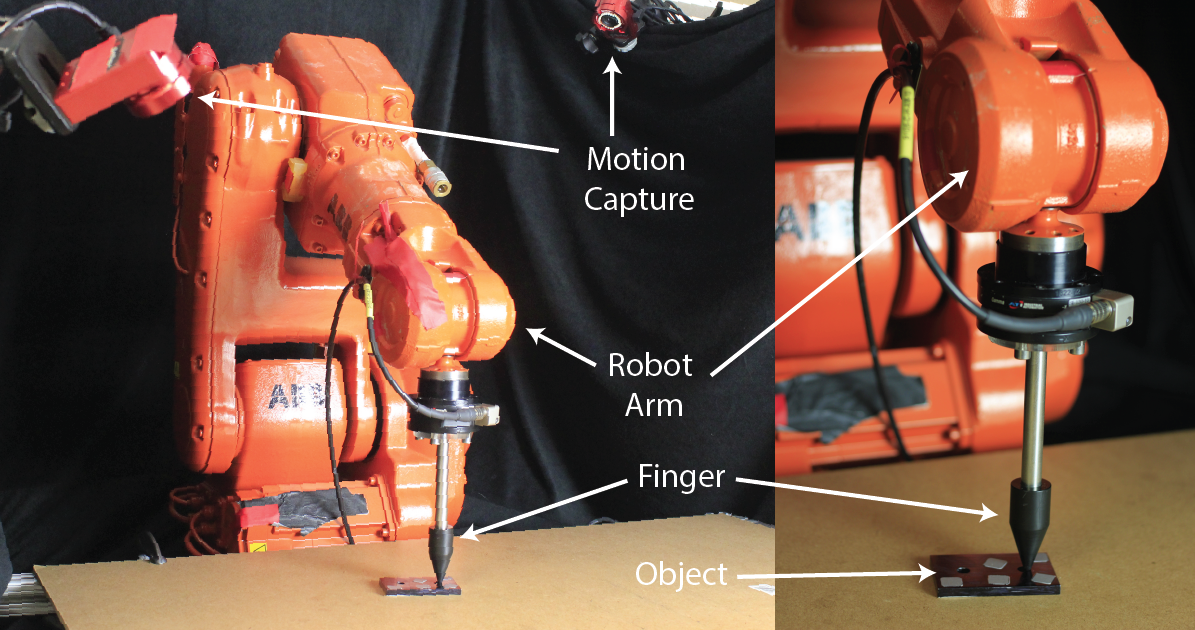
\includegraphics[width=\columnwidth]{fig/hardware.png}
  \end{center}
  \caption{Hardware setup for robotic pulling experiments.}
  \label{fig:hardware}
\end{figure}

Figure \ref{fig:hardware} shows the experimental setup that we used to
test the robotic pulling trajectories generated by the planning
algorithm in Subsection \ref{sec:diff-dynam-progr}.

% With this experiment we aim to test mainly two things:
% \begin{itemize}
% \item the validity of the trajectories generated by the planner, and
% \item convergence of the pulled object to the commanded pose.
% \end{itemize}

Experimental data was collected using an ABB 140 manipulator equipped
with a conical finger. The test object was a laser-cut acrylic
rectangle (75mmx50mmx6.35mm) with 8 holes at the edges and
corners. The conical finger moved the acrylic rectangle by pulling
inside the holes.  A 5 camera OptiTrack motion capture system was set
up to record ground truth position of the object in 2D with a accuracy
of 2mm. To compensate sensing error, the holes on the rectangle were
oversized to have a 3mm radius. We used MDF board as our surface
material.

\begin{figure}
\begin{center}
  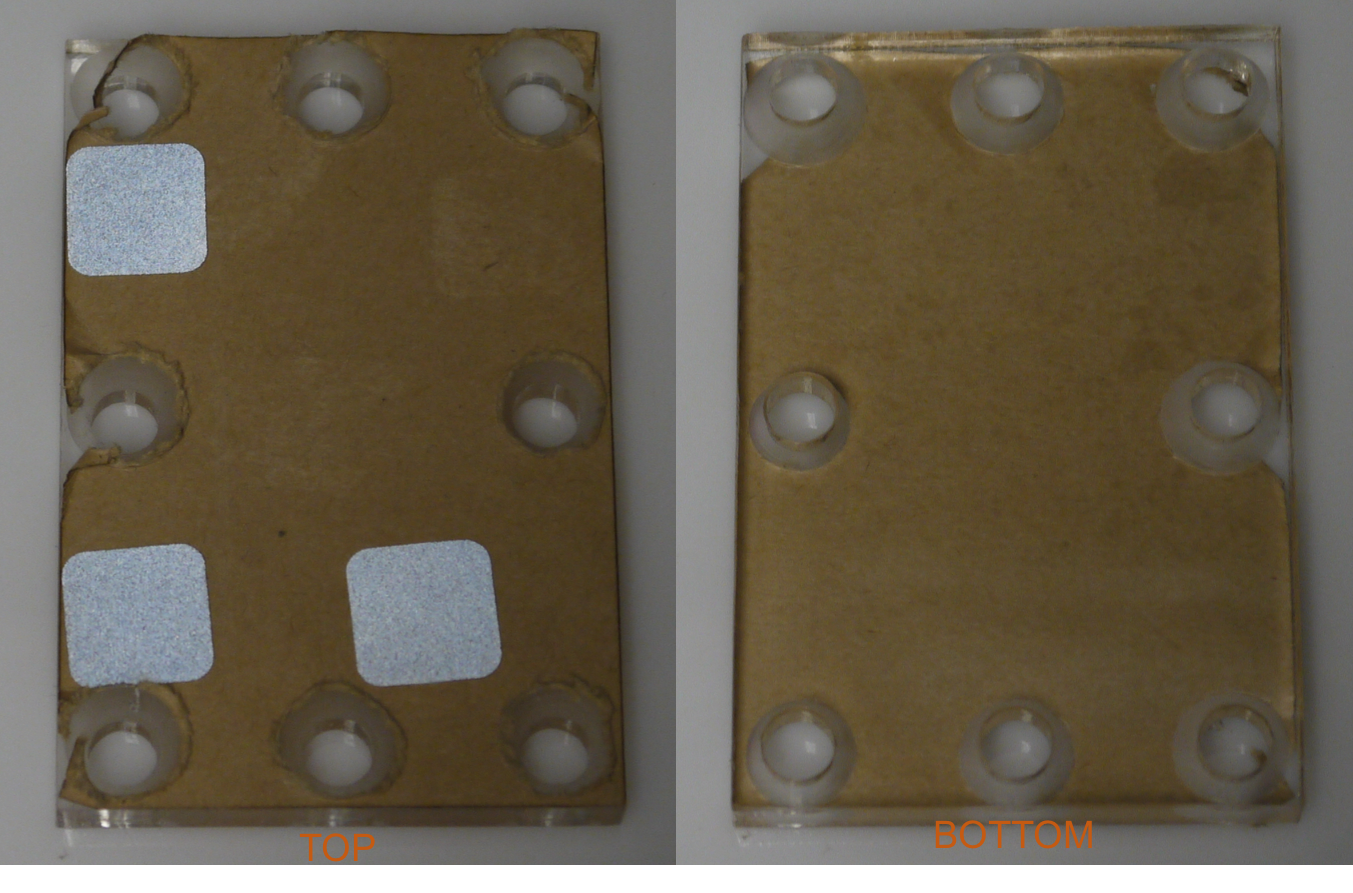
\includegraphics[width=\columnwidth]{fig/object}
\end{center}
\caption{The top and bottom view of the acrylic rectangle with motion
  capture markers and 8 holes for pulling.}
\label{fig:object}
\end{figure}

We computed angular velocity bounds for the acrylic rectangle over
pressure distributions restricted to have at least 25\% of the object
is in contact with the surface. The slope $\mathbf{k}$ of the
Pseudo-Huber Loss function for the DDP planner was set to
$[5000, 5000, 1000, 1000]$ and the width $\bm{\delta}$ was set to
$[0.01, 0.01, 0.02, 0.02]$. The distance penalty $\lambda$ was set to
$40$. For each pulling trial, we generated random start and end poses
within the vision system's field of view. The planner was evaluated
for all eight contact points and the lowest cost trajectory that
remained within the robot workspace was executed on the robot at
25mm/s linear speed. The final pose was then recorded by the motion
capture system.

We collected 80 trials of robotic pulling. Of those, we discarded the
4 trials where the algorithm failed to find any feasible trajectory
within the robot workspace. The average absolute displacement from the
target pose was 4.00mm $\pm$ 3.02mm. The average absolute angular
displacement from the target pose was 4.35 degrees $\pm$ 3.14
degrees. Note the hole radius introduces a systematic error of 3mm to
the final pose because the puller contacts the edge of the hole, not
the center. Overall, our experimental results support the claim that
the planner finds convergent pulling trajectories. An example trial is
visualized in Figure \ref{fig:trajectory}.

% We distinguish between two types of error during the pulling
% experiments. The target error is the error between the target pose and
% the final pose measured by the MoCap. The commanded error is the error
% between the last commanded pose and the final pose measured by the
% MoCap.

% This distinction is important because the target error quantifies the
% performance of our planner, while the commanded error quantifies the
% performance of our theoretical bounds.

% avg_radial_error =
%     0.0040
% std_radial_error =
%     0.0030
% avg_angular_error =
%     4.3457
% std_angular_error =
%     3.1450

% \begin{table}[t]
  % \begin{center}
  %     \begin{tabular}[c]{cccc}
  %       \toprule
  %       & $r$ & $\theta$ \\
  %       \midrule
  %       target & & & \\
  %       \midrule 
  %       command & & & \\
  %       \bottomrule
  %     \end{tabular}
  % \end{center}
  % \caption{Comparison of distance-to-convergence (in meters) for different objects and angular velocity bounds. The top and bottom values in each cell correspond to distances from the upper and lower angular velocity bounds, respectively. See Section \ref{sec:bound-comparison} for the experimental setup.}
% \end{table}

\begin{figure}
\begin{center}
  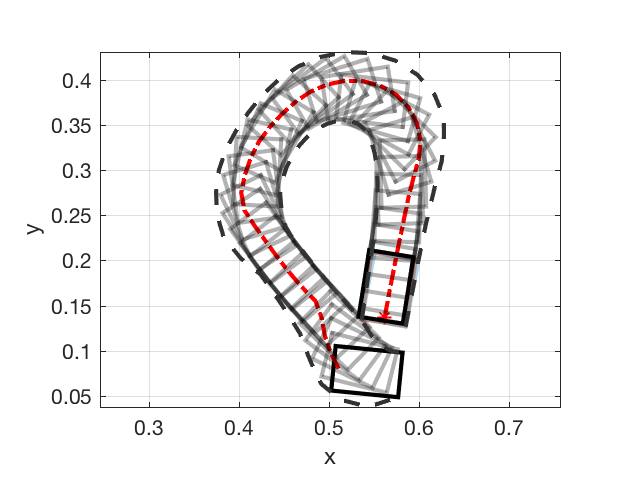
\includegraphics[width=\columnwidth]{fig/trajectory_2.eps}
\end{center}
\caption{(Dashed red line) The planned robotic pulling
  trajectory. (Dashed black line) The area swept by the possible poses
  computed by our bounds during the planned trajectory. (Grey
  rectangles) The measured poses of the object when the trajectory was
  executed on a real robot.}
\label{fig:trajectory}
\end{figure}

% \section{Discussion}\label{sec:discussion}
\section{Conclusion}\label{sec:conclusion}

In this paper, we derive a method for computing exact bounds on the
object's motion for classes of pressure distributions where the center
of pressure is known but the distribution of support forces is
unknown. We also show these exact motion bounds can be used to plan
robotic pulling trajectories that guarantee the pulled object
converges to the final pose. We validate our planner on a real robotic
system and show that the generated trajectories obtain low errors on
the final pose of the object.

\bibliographystyle{plainnat}
\bibliography{references}

\end{document}


